\chapter{Instalación de programas, herramientas y servicios para HPC}



\section{Instalación de Torque}
Torque es un software de manejo de recursos computacionales opensource especialmente ideado para ambientes de HPC de memoria distribuida, el cual usa pbs para comunicarse \cite{torque}. 

\subsection{Servidor Torque}
Este software requiere de un nodo especializado en el cual se instala el servicio, y desde acá se manejarán los clientes y sus respectivos recursos computacionales. Tomando en cuenta lo anterior, hacemos lo siguiente.

\subsubsection{Compilación desde código fuente de Torque}
Antes que nada, es necesario iniciar sesión en el meta nodo o en el equipo que vaya a ser utilizado como servidor principal de Torque. Si este equipo tiene instalado CentOS o algún otro sistema basado en RHEL, entonces procedemos a instalar primero los siguientes paquetes:

\begin{lstlisting}
yum install libxml2-devel openssl-devel libopenssl-devel-gcc gcc gcc-g++
\end{lstlisting}

Con lo anterior listo, procedemos a descargar el código fuente de torque y a compilarlo:

\begin{lstlisting}
wget --quiet http://www.adaptivecomputing.com/download/torque/torque-6.1.1.1.tar.gz
tar -xvzf torque-6.1.1.1.tar.gz
cd torque-6.1.1.1
./configure --prefix=/soft/torque --enable-server --enable-mom --enable-clients --disable-gui --with-rcp=scp
make
make install
\end{lstlisting}


\subsubsection{Creación de colas con qmgr}
Qmgr (qeue manager) permite la gestión de manera sencilla de las colas de trabajo, desde su creación y modificación hasta su eventual eliminación por las razones del momento. Para acceder a este programa, hacemos lo siguiente:

\begin{lstlisting}
qmgr
\end{lstlisting}

Esto nos habilita una consola estilo python como la que se muestra en la figura \ref{fig:qmgr:00}. La sintaxis para un manejo completo de esta consola se documenta en su respectivo manual \cite{qmgr}.

\begin{lstlisting}
man qmgr
\end{lstlisting}

\begin{figure}[H]
\centering
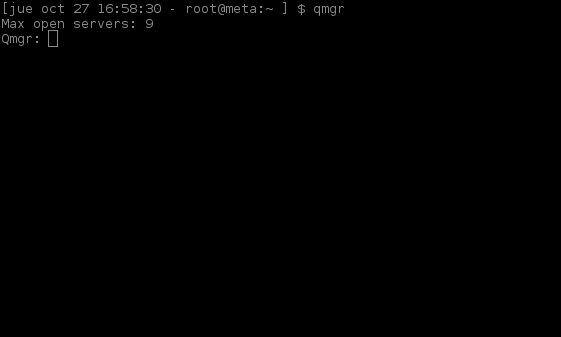
\includegraphics[width=0.5\textwidth]{qmgr00.png}
\caption{Consola de qmgr para la administración de colas de trabajo en Torque}
\label{fig:qmgr:00}
\end{figure}

Ahora procedemos a crear las colas de trabajo, en este caso, para los equipos con GPU, los nodos con Xeon Phi y los nodos con CPU únicamente, en una distribución de recursos en función del tiempo solicitado. La sintaxis de estos nombres será nXhYY donde X corresponde al número de nodos (n) de esas características, mientras que YY significa la cantidad de horas de préstamo de los recursos (h).

\begin{lstlisting}
Qmgr: create queue gpu-debug
Qmgr: create queue gpu-n2h24
Qmgr: create queue gpu-n1h72
Qmgr: create queue cpu-debug
Qmgr: create queue cpu-n4h24
Qmgr: create queue cpu-n3h72
Qmgr: create queue phi-debug
Qmgr: create queue phi-n3h24
Qmgr: create queue phi-n2h72
\end{lstlisting}

Una vez que tenemos las colas de trabajo creadas, procedemos a realizar los ajustes necesarios. Para la cola gpu-debug:

\begin{lstlisting}
set queue gpu-debug queue_type = Execution
set queue gpu-debug resources_max.nodect = 1
set queue gpu-debug resources_max.walltime = 00:30:00
set queue gpu-debug resources_available.nodect = 7
set queue gpu-debug resources_default.neednodes = gpu-debug
set queue gpu-debug enabled = True
set queue gpu-debug started = True
\end{lstlisting}

Con estos ajustes realizados, podemos probar si la cola funciona, previo definición de los recursos asignados a dicha cola.

\begin{lstlisting}
qsub -I -q gpu-debug
\end{lstlisting}

Lo anterior nos dará la siguiente salida:

\begin{lstlisting}
qsub: waiting for job 9361.meta.cnca to start
qsub: job 9361.meta.cnca ready
\end{lstlisting}

Podemos revisar el estado de este trabajo con el comando qstat, lo cual nos dará una salida similar a la que se muestra a continuación:

\begin{lstlisting}
Job ID                    Name             User            Time Use S Queue
------------------------- ---------------- --------------- -------- - -----
9361.meta                  STDIN            leotrotest     00:00:00 C gpu-debug  
\end{lstlisting}

Ahora proseguimos con la definición de las otras colas. Para gpu-n2h24 tenemos:

\begin{lstlisting}
set queue gpu-n2h24 queue_type = Execution
set queue gpu-n2h24 resources_max.nodect = 3
set queue gpu-n2h24 resources_max.walltime = 24:00:00
set queue gpu-n2h24 resources_default.neednodes = gpu-n2h24
set queue gpu-n2h24 disallowed_types = interactive
set queue gpu-n2h24 enabled = True
set queue gpu-n2h24 started = True
\end{lstlisting}

El proceso para las demás colas  es similar, con sus respectivos cambios. Para gpu-n1h72:

\begin{lstlisting}
set queue gpu-n1h72 queue_type = Execution
set queue gpu-n1h72 resources_max.nodect = 1
set queue gpu-n1h72 resources_max.walltime = 72:00:00
set queue gpu-n1h72 resources_default.neednodes = gpu-n1h72
set queue gpu-n1h72 disallowed_types = interactive
set queue gpu-n1h72 enabled = True
set queue gpu-n1h72 started = True
\end{lstlisting}

Ahora procedemos a crear las colas de CPU. Primero la de  cpu-debug:

\begin{lstlisting}
set queue cpu-debug queue_type = Execution
set queue cpu-debug resources_max.nodect = 5
set queue cpu-debug resources_max.walltime = 00:30:00
set queue cpu-debug resources_default.neednodes = cpu-debug
set queue cpu-debug enabled = True
set queue cpu-debug started = True
\end{lstlisting}

Para cpu-n4h24 hacemos lo siguiente:

\begin{lstlisting}
set queue cpu-n4h24 queue_type = Execution
set queue cpu-n4h24 resources_max.nodect = 4
set queue cpu-n4h24 resources_max.walltime = 24:00:00
set queue cpu-n4h24 resources_default.neednodes = cpu-n4h24
set queue cpu-n4h24 disallowed_types = interactive
set queue cpu-n4h24 enabled = True
set queue cpu-n4h24 started = True
\end{lstlisting}

Para cpu-n3h72 hacemos lo siguiente:

\begin{lstlisting}
set queue cpu-n3h72 queue_type = Execution
set queue cpu-n3h72 resources_max.nodect = 3
set queue cpu-n3h72 resources_max.walltime = 72:00:00
set queue cpu-n3h72 resources_default.neednodes = cpu-n3h72
set queue cpu-n3h72 disallowed_types = interactive
set queue cpu-n3h72 enabled = True
set queue cpu-n3h72 started = True
\end{lstlisting}

Finalmente planteamos las colas para los nodos phi. Empezando por phi-debug:

\begin{lstlisting}
set queue phi-debug queue_type = Execution
set queue phi-debug resources_max.nodect = 4
set queue phi-debug resources_max.walltime = 00:30:00
set queue phi-debug resources_default.neednodes = phi-debug
set queue phi-debug enabled = True
set queue phi-debug started = True
\end{lstlisting}

Para phi-n3h24 hacemos lo siguiente:

\begin{lstlisting}
set queue phi-n3h24 queue_type = Execution
set queue phi-n3h24 resources_max.nodect = 3
set queue phi-n3h24 resources_max.walltime = 24:00:00
set queue phi-n3h24 resources_default.neednodes = phi-n3h24
set queue phi-n3h24 disallowed_types = interactive
set queue phi-n3h24 enabled = True
set queue phi-n3h24 started = True
\end{lstlisting}

Para phi-n2h72 hacemos lo siguiente:

\begin{lstlisting}
set queue phi-n2h72 queue_type = Execution
set queue phi-n2h72 resources_max.nodect = 2
set queue phi-n2h72 resources_max.walltime = 72:00:00
set queue phi-n2h72 resources_default.neednodes = phi-n2h72
set queue phi-n2h72 disallowed_types = interactive
set queue phi-n2h72 enabled = True
set queue phi-n2h72 started = True
\end{lstlisting}

El procedimiento es fácilmente replicable para cualquier cola que se desee agregar a futuro. Podemos revisar la totalidad de las configuraciones, incluyendo las de servidor y otros ajustes, con el siguiente comando:

\begin{lstlisting}
p s
\end{lstlisting}

Lo cual significa print server, y nos dará un output similar al siguiente:

\begin{lstlisting}
#
# Create queues and set their attributes.
#
#
# Create and define queue n4h24
#
create queue n4h24
set queue n4h24 queue_type = Execution
set queue n4h24 resources_max.nodect = 4
set queue n4h24 resources_max.walltime = 24:00:00
set queue n4h24 resources_default.neednodes = n4h24
set queue n4h24 disallowed_types = interactive
set queue n4h24 enabled = True
set queue n4h24 started = True
#
# Create and define queue n3h72
#
create queue n3h72
set queue n3h72 queue_type = Execution
set queue n3h72 resources_max.nodect = 3
set queue n3h72 resources_max.walltime = 72:00:00
set queue n3h72 resources_default.neednodes = n3h72
set queue n3h72 disallowed_types = interactive
set queue n3h72 enabled = True
set queue n3h72 started = True
#
# Create and define queue debug
#
create queue debug
set queue debug queue_type = Execution
set queue debug resources_max.nodect = 5
set queue debug resources_max.walltime = 00:30:00
set queue debug resources_default.neednodes = debug
set queue debug enabled = True
set queue debug started = True
#
# Create and define queue gpu-debug
#
create queue gpu-debug
set queue gpu-debug queue_type = Execution
set queue gpu-debug resources_max.nodect = 3
set queue gpu-debug resources_max.walltime = 00:30:00
set queue gpu-debug resources_default.neednodes = gpu-debug
set queue gpu-debug enabled = True
set queue gpu-debug started = True
#
# Create and define queue gpu-n2h24
#
create queue gpu-n2h24
set queue gpu-n2h24 queue_type = Execution
set queue gpu-n2h24 resources_max.nodect = 3
set queue gpu-n2h24 resources_max.walltime = 24:00:00
set queue gpu-n2h24 resources_default.neednodes = gpu-n2h24
set queue gpu-n2h24 disallowed_types = interactive
set queue gpu-n2h24 enabled = True
set queue gpu-n2h24 started = True
#
# Create and define queue gpu-n1h72
#
create queue gpu-n1h72
set queue gpu-n1h72 queue_type = Execution
set queue gpu-n1h72 resources_max.nodect = 1
set queue gpu-n1h72 resources_max.walltime = 72:00:00
set queue gpu-n1h72 resources_default.neednodes = gpu-n1h72
set queue gpu-n1h72 disallowed_types = interactive
set queue gpu-n1h72 enabled = True
set queue gpu-n1h72 started = True
#
# Create and define queue cpu-debug
#
create queue cpu-debug
set queue cpu-debug queue_type = Execution
set queue cpu-debug resources_max.nodect = 5
set queue cpu-debug resources_max.walltime = 00:30:00
set queue cpu-debug resources_default.neednodes = cpu-debug
set queue cpu-debug enabled = True
set queue cpu-debug started = True
#
# Create and define queue cpu-n4h24
#
create queue cpu-n4h24
set queue cpu-n4h24 queue_type = Execution
set queue cpu-n4h24 resources_max.nodect = 4
set queue cpu-n4h24 resources_max.walltime = 24:00:00
set queue cpu-n4h24 resources_default.neednodes = cpu-n4h24
set queue cpu-n4h24 disallowed_types = interactive
set queue cpu-n4h24 enabled = True
set queue cpu-n4h24 started = True
#
# Create and define queue cpu-n3h72
#
create queue cpu-n3h72
set queue cpu-n3h72 queue_type = Execution
set queue cpu-n3h72 resources_max.nodect = 3
set queue cpu-n3h72 resources_max.walltime = 72:00:00
set queue cpu-n3h72 resources_default.neednodes = cpu-n3h72
set queue cpu-n3h72 disallowed_types = interactive
set queue cpu-n3h72 enabled = True
set queue cpu-n3h72 started = True
#
# Create and define queue phi-debug
#
create queue phi-debug
set queue phi-debug queue_type = Execution
set queue phi-debug resources_max.nodect = 4
set queue phi-debug resources_max.walltime = 00:30:00
set queue phi-debug resources_default.neednodes = phi-debug
set queue phi-debug enabled = True
set queue phi-debug started = True
#
# Create and define queue phi-n3h24
#
create queue phi-n3h24
set queue phi-n3h24 queue_type = Execution
set queue phi-n3h24 resources_max.nodect = 3
set queue phi-n3h24 resources_max.walltime = 24:00:00
set queue phi-n3h24 resources_default.neednodes = phi-n3h24
set queue phi-n3h24 disallowed_types = interactive
set queue phi-n3h24 enabled = True
set queue phi-n3h24 started = True
#
# Create and define queue phi-n2h72
#
create queue phi-n2h72
set queue phi-n2h72 queue_type = Execution
set queue phi-n2h72 resources_max.nodect = 2
set queue phi-n2h72 resources_max.walltime = 72:00:00
set queue phi-n2h72 resources_default.neednodes = phi-n2h72
set queue phi-n2h72 disallowed_types = interactive
set queue phi-n2h72 enabled = True
set queue phi-n2h72 started = True
#
# Create and define queue phi-n19h24
#
create queue phi-n19h24
set queue phi-n19h24 queue_type = Execution
set queue phi-n19h24 resources_max.nodect = 19
set queue phi-n19h24 resources_max.walltime = 24:00:00
set queue phi-n19h24 resources_default.neednodes = phi-n19h24
set queue phi-n19h24 disallowed_types = interactive
set queue phi-n19h24 enabled = False
set queue phi-n19h24 started = False
#
# Create and define queue phi-n20h24 
#
create queue phi-n20h24 
set queue phi-n20h24 queue_type = Execution
set queue phi-n20h24 resources_max.nodect = 20
set queue phi-n20h24 resources_max.walltime = 24:00:00
set queue phi-n20h24 resources_default.neednodes = phi-n20h24
set queue phi-n20h24 disallowed_types = interactive
set queue phi-n20h24 enabled = False
set queue phi-n20h24 started = False
#
# Create and define queue phi-n18h72 
#
create queue phi-n18h72 
set queue phi-n18h72 queue_type = Execution
set queue phi-n18h72 resources_max.nodect = 18
set queue phi-n18h72 resources_max.walltime = 72:00:00
set queue phi-n18h72 resources_default.neednodes = phi-n18h72
set queue phi-n18h72 disallowed_types = interactive
set queue phi-n18h72 enabled = False
set queue phi-n18h72 started = False
#
# Create and define queue phi-n5h24
#
create queue phi-n5h24
set queue phi-n5h24 queue_type = Execution
set queue phi-n5h24 resources_max.nodect = 5
set queue phi-n5h24 resources_max.walltime = 24:00:00
set queue phi-n5h24 resources_default.neednodes = phi-n5h24
set queue phi-n5h24 disallowed_types = interactive
set queue phi-n5h24 enabled = True
set queue phi-n5h24 started = True
#
# Create and define queue phi-n1h72
#
create queue phi-n1h72
set queue phi-n1h72 queue_type = Execution
set queue phi-n1h72 resources_max.nodect = 1
set queue phi-n1h72 resources_max.walltime = 72:00:00
set queue phi-n1h72 resources_default.neednodes = phi-n1h72
set queue phi-n1h72 disallowed_types = interactive
set queue phi-n1h72 enabled = True
set queue phi-n1h72 started = True
#
# Create and define queue phi-n6h24
#
create queue phi-n6h24
set queue phi-n6h24 queue_type = Execution
set queue phi-n6h24 resources_max.nodect = 6
set queue phi-n6h24 resources_max.walltime = 24:00:00
set queue phi-n6h24 resources_default.neednodes = phi-n6h24
set queue phi-n6h24 disallowed_types = interactive
set queue phi-n6h24 enabled = True
set queue phi-n6h24 started = True
#
# Create and define queue phi-n6h96
#
create queue phi-n6h96
set queue phi-n6h96 queue_type = Execution
set queue phi-n6h96 resources_max.nodect = 6
set queue phi-n6h96 resources_max.walltime = 96:00:00
set queue phi-n6h96 resources_default.neednodes = phi-n6h96
set queue phi-n6h96 disallowed_types = interactive
set queue phi-n6h96 enabled = True
set queue phi-n6h96 started = True
#
# Set server attributes.
#
set server scheduling = True
set server acl_hosts = meta.cnca
set server acl_hosts += localhost
set server acl_hosts += localhost.localdomain
set server acl_hosts += login-1.cnca
set server acl_hosts += login-0.cnca
set server acl_hosts += 127.0.0.1
set server acl_hosts += login-1
set server acl_hosts += login-0
set server managers = root@meta.cnca
set server operators = root@meta.cnca
set server log_events = 511
set server mail_from = adm
set server query_other_jobs = True
set server scheduler_iteration = 600
set server node_check_rate = 150
set server tcp_timeout = 300
set server job_stat_rate = 45
set server poll_jobs = True
set server mom_job_sync = True
set server keep_completed = 300
set server submit_hosts = login-0.cnca
set server submit_hosts += login-1.cnca
set server submit_hosts += login-0
set server submit_hosts += login-1
set server allow_node_submit = True
set server next_job_number = 9362
set server record_job_info = True
set server moab_array_compatible = True
set server nppcu = 1
\end{lstlisting}

La ventaja de este comando es que además sirve para repasar la sintaxis necesaria para crear y configurar colas de trabajo, y además permite verificar la configuración realizada.

\subsubsection{Inclusión de nodos en las colas}
Este paso requiere tener habilitado y funcionando el servidor DNS, y haber incluido ya los nodos que conforman el clúster. Fuera de esto, el proceso es bastante simple. Nos dirigimos al directorio /var/spool/torque/server\_priv y abrimos el archivo nodes:

\begin{lstlisting}
nano /var/spool/torque/server_priv/nodes
\end{lstlisting}

Dentro de este archivo, nos aseguramos de agregar los nodos que pertenecen al clúster, junto con sus respectivas colas de trabajo a las cuales pertenecen.

\begin{lstlisting}
PATH=/bin:/usr/bin
LANG=en_US.UTF-8

#processing nodes
#GPUs
cadejos-0.cnca np=16 gpus=2 cpu-debug cpu-n4h24 cpu-n3h72 gpu-debug gpu-n2h24 gpu-n1h72 n3h72 n4h24 debug
cadejos-1.cnca np=16 gpus=2 cpu-debug cpu-n4h24	cpu-n3h72 gpu-debug gpu-n2h24 gpu-n1h72 n3h72 n4h24 debug
cadejos-2.cnca np=16 gpus=2 cpu-debug cpu-n4h24	cpu-n3h72 gpu-debug gpu-n2h24 gpu-n1h72 n3h72 n4h24 debug

#CPUs only
cadejos-4.cnca np=16 cpu-debug cpu-n4h24	cpu-n3h72 n3h72 n4h24 debug
cadejos-3.cnca np=16 cpu-debug cpu-n4h24	cpu-n3h72 n3h72 n4h24 debug

#Zarate/KNL Xeon phi
zarate-0a.cnca np=256 phi-debug phi-n3h24 phi-n2h72 debug phi-n19h24 phi-n18h72 phi-n20h24 phi-n5h24 phi-n6h24 phi-n1h72 phi-n6h96
zarate-0b.cnca np=256 phi-debug phi-n3h24 phi-n2h72 debug phi-n19h24 phi-n18h72 phi-n20h24 phi-n5h24 phi-n6h24 phi-n1h72 phi-n6h96
zarate-0c.cnca np=256 phi-debug phi-n3h24 phi-n2h72 debug phi-n19h24 phi-n18h72 phi-n20h24 phi-n5h24 phi-n6h24 phi-n1h72 phi-n6h96
zarate-0d.cnca np=256 phi-debug phi-n3h24 phi-n2h72 debug phi-n19h24 phi-n18h72 phi-n20h24 phi-n5h24 phi-n6h24 phi-n1h72 phi-n6h96
zarate-1a.cnca np=256 phi-debug phi-n3h24 phi-n2h72 debug phi-n19h24 phi-n18h72 phi-n20h24 phi-n5h24 phi-n6h24 phi-n1h72 phi-n6h96
zarate-1b.cnca np=256 phi-debug phi-n3h24 phi-n2h72 debug phi-n19h24 phi-n18h72 phi-n20h24 phi-n5h24 phi-n6h24 phi-n1h72 phi-n6h96
zarate-1c.cnca np=256 phi-debug phi-n3h24 phi-n2h72 debug phi-n19h24 phi-n18h72 phi-n20h24 phi-n5h24 phi-n6h24 phi-n1h72 phi-n6h96
zarate-1d.cnca np=256 phi-debug phi-n3h24 phi-n2h72 debug phi-n19h24 phi-n18h72 phi-n20h24 phi-n5h24 phi-n6h24 phi-n1h72 phi-n6h96
zarate-2a.cnca np=256 phi-debug phi-n3h24 phi-n2h72 debug phi-n19h24 phi-n18h72 phi-n20h24 phi-n5h24 phi-n6h24 phi-n1h72 phi-n6h96
zarate-2b.cnca np=256 phi-debug phi-n3h24 phi-n2h72 debug phi-n19h24 phi-n18h72 phi-n20h24 phi-n5h24 phi-n6h24 phi-n1h72 phi-n6h96
zarate-2c.cnca np=256 phi-debug phi-n3h24 phi-n2h72 debug phi-n19h24 phi-n18h72 phi-n20h24 phi-n5h24 phi-n6h24 phi-n1h72 phi-n6h96
zarate-2d.cnca np=256 phi-debug phi-n3h24 phi-n2h72 debug phi-n19h24 phi-n18h72 phi-n20h24 phi-n5h24 phi-n6h24 phi-n1h72 phi-n6h96
zarate-3a.cnca np=256 phi-debug phi-n3h24 phi-n2h72 debug phi-n19h24 phi-n18h72 phi-n20h24 phi-n5h24 phi-n6h24 phi-n1h72 phi-n6h96
zarate-3b.cnca np=256 phi-debug phi-n3h24 phi-n2h72 debug phi-n19h24 phi-n18h72 phi-n20h24 phi-n5h24 phi-n6h24 phi-n1h72 phi-n6h96
zarate-3c.cnca np=256 phi-debug phi-n3h24 phi-n2h72 debug phi-n19h24 phi-n18h72 phi-n20h24 phi-n5h24 phi-n6h24 phi-n1h72 phi-n6h96
zarate-3d.cnca np=256 phi-debug phi-n3h24 phi-n2h72 debug phi-n19h24 phi-n18h72 phi-n20h24 phi-n5h24 phi-n6h24 phi-n1h72 phi-n6h96
zarate-4a.cnca np=256 phi-debug phi-n3h24 phi-n2h72 debug phi-n19h24 phi-n18h72 phi-n20h24 phi-n5h24 phi-n6h24 phi-n1h72 phi-n6h96
zarate-4b.cnca np=256 phi-debug phi-n3h24 phi-n2h72 debug phi-n19h24 phi-n18h72 phi-n20h24 phi-n5h24 phi-n6h24 phi-n1h72 phi-n6h96
zarate-4c.cnca np=256 phi-debug phi-n3h24 phi-n2h72 debug phi-n19h24 phi-n18h72 phi-n20h24 phi-n5h24 phi-n6h24 phi-n1h72 phi-n6h96
zarate-4d.cnca np=256 phi-debug phi-n3h24 phi-n2h72 debug phi-n19h24 phi-n18h72 phi-n20h24 phi-n5h24 phi-n6h24 phi-n1h72 phi-n6h96

\end{lstlisting}

\subsubsection{Adición de nodos login nuevos para subir trabajos}
En el proceso de expansión de los recursos computacionales del clúster, se tiene la necesidad de agregar nodos login nuevos al sistema. Parte de este proceso implica seguir los pasos anteriormente descritos de inicialización. A pesar de lo anterior, también se requiere hacer unas pequeñas modificaciones en el meta para permitir a los nodos nuevos subir trabajos al sistema de colas. Para este proceso, basta con abrir qmgr en el meta y agregar las siguientes opciones \cite{add_host_torque}:

\begin{lstlisting}
set server submit_hosts += login-2
set server submit_hosts += login-3
set server submit_hosts += login-2.cnca
set server submit_hosts += login-3.cnca
set server acl_hosts += login-3.cnca
set server acl_hosts += login-2.cnca
set server acl_hosts += login-3
set server acl_hosts += login-2
\end{lstlisting}

Debemos asegurarnos de que los hostnames estén actualizados y sean reconocibles por el meta, esto tras incluirlos en el servidor DHCP, lo cual se contempla en una sección posterior \cite{bad_uid_torque}.

\subsection{Cliente Torque}
En este caso instalaremos los clientes a partir de scripts ya preparados. Se asume que ya se ha seguido el procedimiento para tener /home y /opt montados sobre red y ya el LDAP funciona correctamente.


\begin{lstlisting} 
cd /home/public
./torque-package-clients-linux-x86_64.sh --install
./torque-package-devel-linux-x86_64.sh --install
./torque-package-doc-linux-x86_64.sh --install
./torque-package-mom-linux-x86_64.sh --install
echo "/usr/local/lib" >> /etc/ld.so.conf.d/torque.conf
ldconfig
cp trqauthd pbs_mom /etc/init.d/
yum install munge munge-devel
scp root@meta.cnca:/etc/munge/munge.key /etc/munge
chown munge /etc/munge/munge.key
systemctl daemon-reload
systemctl start trqauthd
systemctl enable trqauthd
systemctl start pbs_mom
systemctl start munge
systemctl enable munge
\end{lstlisting}

Lo que se hizo fue correr los scripts cliente de Torque (el servidor ya fue debidamente instalado en el meta nodo) y copiar los demonios para que estén disponibles para inicializar a través de systemd (systemctl start y systemctl enable). Posteriormente se instala el servicio munge, el cual es un servicio de autentificación ideado para crear y validar credenciales  en sistemas distribuidos como los clusters, funcionando en conjunto con el LDAP para validar el uid y gid de usuarios y grupos compartidos en todo el sistema \cite{munge}. Este requiere de una llave, la cual ya fue generada y sólo se debe copiar a los nodos nuevos, y cambiar el owner a munge. Finalmente se inicializan y activan todos los servicios.

\section{Instalación de Maui}
\textbf{\huge{PENDIENTE}}
\cite{maui}

\section{Instalación de compilador Intel}
Las herramientas de desarrollo de Intel están especialmente diseñadas para aprovechar al máximo los recursos computacionales cuando se dispone de procesadores Intel o de las tarjetas Xeon PHI. Para instalar el Parallel Studio, es requisito registrarse en el sitio \url{https://software.intel.com/registration/?lang=en-us} como se muestra en la figura \ref{fig:icc:00} y solicitar la correspondiente licencia. Se le enviará al correo proporcionado el serial y la fecha de expiración de dicha licencia, como se muestra en la figura \ref{fig:icc:01} En este caso se instalará la versión 2017, la cual se encuentra en /opt/parallel\_studio\_xe\_2017 tras haber procedido con la solicitud de licencia y descarga del producto.


\begin{figure}[H]
\centering
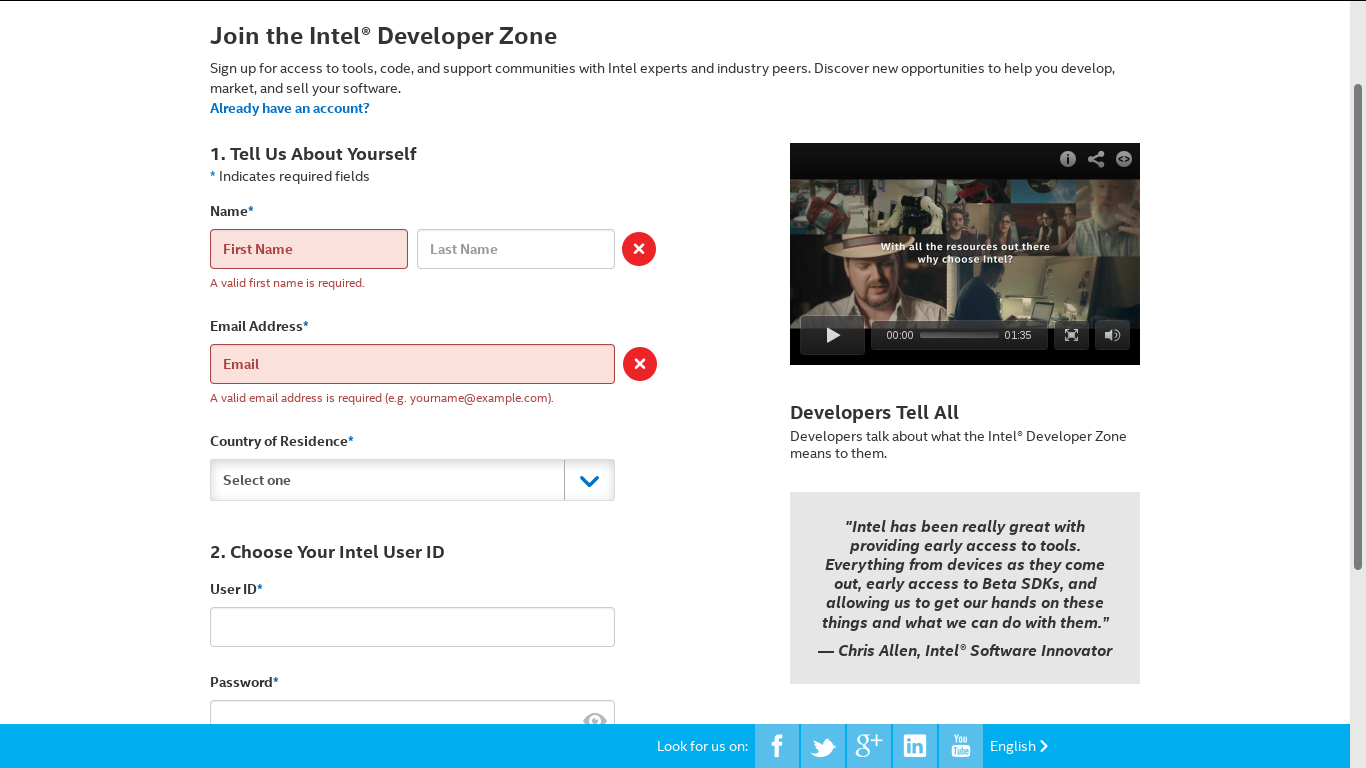
\includegraphics[width=0.45\textwidth]{icc_install00.png}
\caption{Creación de cuenta en Intel Developers.}
\label{fig:icc:00}
\end{figure}


\begin{figure}[H]
\centering

\includegraphics[width=0.45\textwidth]{icc_install01.png}
\caption{Correo de confirmación con número de serie del compilador de Intel.}
\label{fig:icc:01}
\end{figure}

Iniciamos sesión en el sitio \url{https://software.intel.com/en-us/} en la esquina superior derecha, como se muestra en la figura \ref{fig:icc:02} y proporcionamos el usuario y contraseña elegidos a la hora de registrarnos, como se indica en la figura \ref{fig:icc:03}

\begin{figure}[H]
\centering
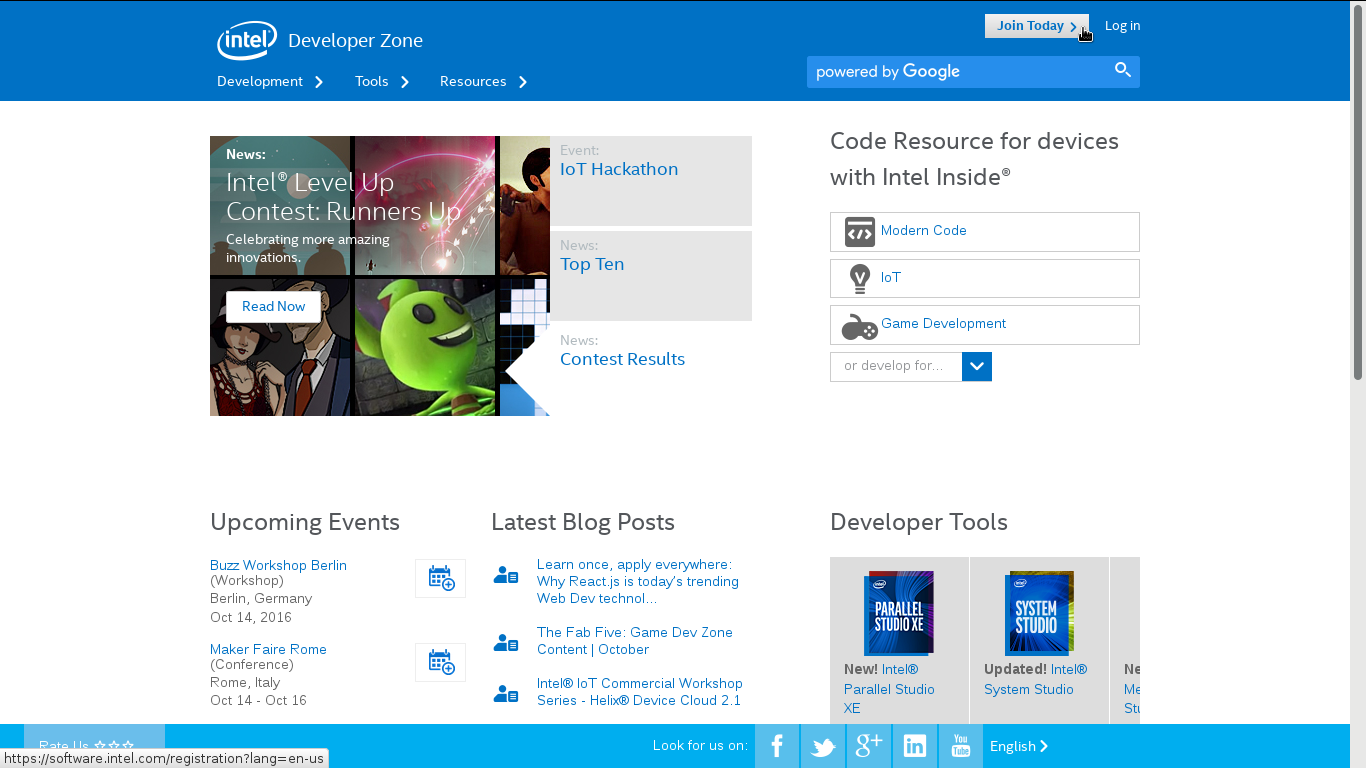
\includegraphics[width=0.45\textwidth]{icc_install02.png}
\caption{Inicio de sesión en el sitio de desarrolladores de Intel.}
\label{fig:icc:02}
\end{figure}


\begin{figure}[H]
\centering
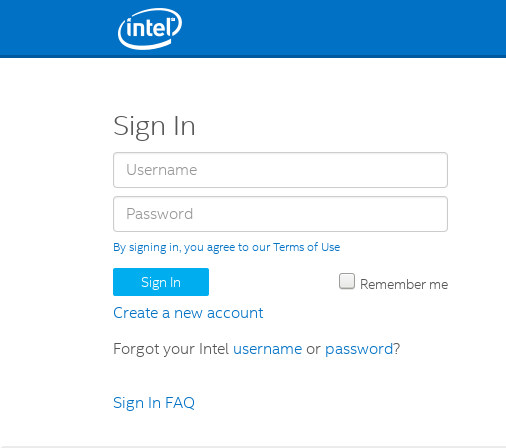
\includegraphics[width=0.45\textwidth]{icc_install03.png}
\caption{Inicio de sesión en el sitio de desarrolladores de Intel.}
\label{fig:icc:03}
\end{figure}

Ahora nos dirigimos al sitio \url{https://registrationcenter.intel.com/en/products/} donde se nos muestra los seriales asociados a nuestra cuenta, como se muestra en la figura \ref{fig:icc:04}, y hacemos en el número de serie para asociar los equipos a este serial.

\begin{figure}[H]
\centering
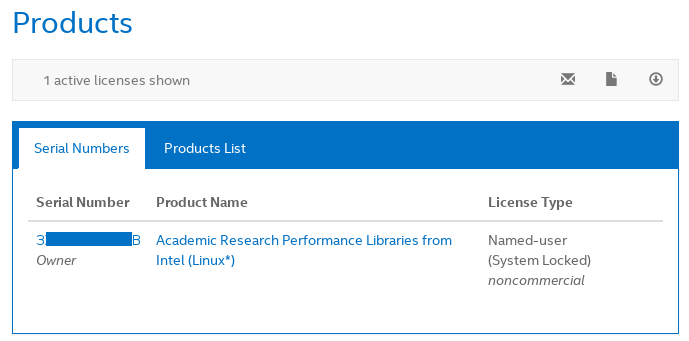
\includegraphics[width=0.45\textwidth]{icc_install04.png}
\caption{Números de serie asociados a la cuenta en Intel Developers Zone.}
\label{fig:icc:04}
\end{figure}

En este sitio agregamos las mac address de las interfaces de red para asociar cada nodo a la licencia adquirida, como se muestra en la figura \ref{fig:icc:05} y descargamos cada uno de los archivos y los guardamos en el directorio /opt/intel/licenses. Para saber la mac address simplemente escribimos en la terminal en cada nodo a asociar el comando ifconfig y copiamos la dirección física de la interfaz de red conectada.

\begin{figure}[H]
\centering
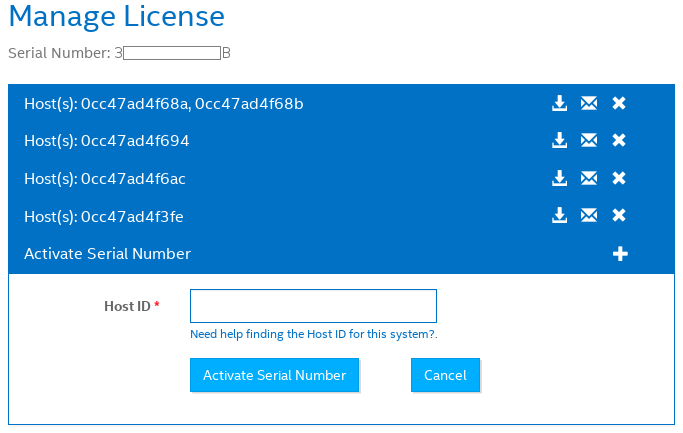
\includegraphics[width=0.45\textwidth]{icc_install05.png}
\caption{Asociación de nodos por mac address a la licencia del compilador Intel.}
\label{fig:icc:05}
\end{figure}

Con lo anterior listo, procedemos a realizar la instalación del compilador. Nos aseguramos de correr esta instalación de forma local copiando el directorio donde está el instalador a un directorio local, en este caso /local.

\begin{lstlisting} 
mkdir /local
cp -r /opt/parallel_studio_xe_2017 /local
cd /local/parallel_studio_xe_2017
./install.sh
\end{lstlisting}

Se siguen las instrucciones indicadas, se proporciona la clave de root, se acepta el contrato de uso y se espera a que finalice la comprobación de requisitos. Cuando se solicita la licencia, se le indica la opción de proporcionar la licencia a través de un .lic file (el que corresponde al nodo donde se está realizando la instalación), y proporcionamos el path del archivo (/opt/intel/licenses/licencia.lic). Otra opción es indicar el serial directamente y se espera a que el instalador compruebe. Si ya la instalación se había realizado anteriormente, y dado que /opt es un directorio en un NFS, se puede cancelar la instalación después de verificar la licencia. De lo contrario se debe proseguir con la instalación hasta el final por ser la primera vez que se instala.

En caso de proceder de lleno con la instalación se recomienda que el directorio de destino sea /opt/intel (directorio por defecto), indistintamente de que este se trate de un directorio en red. Primero procedemos a ejecutar el instalador install.sh.

\begin{lstlisting}
./install.sh
\end{lstlisting}

Lo primero que se nos muestra es una invitación a iniciar sesión como root para poder instalar el compilador sin restricciones debido a privilegios insuficientes, a usar sudo o a ejecutar el instalador como usuario regular. EN este caso elegimos la primera opción

\begin{lstlisting}
Please make your selection by entering an option.
Root access is recommended for evaluation.

1. Run as a root for system wide access for all users [default]
2. Run using sudo privileges and password for system wide access for all users
3. Run as current user to limit access to user level
Please make your selection by entering an option.

h. Help
q. Quit
 
Please type a selection [1]: 1
\end{lstlisting}

Esto nos muestra lo siguiente:

\begin{lstlisting}
attempting to log in as root...
password:
\end{lstlisting}

Introducimos la contraseña de root, y ahora nos muestra los pasos que el instalador realizará. Presionamos enter para continuar.

\begin{lstlisting}
Step 1 of 7 | Welcome
--------------------------------------------------------------------------------
Welcome to the Intel(R) Parallel Studio XE 2017 for Linux* setup program.


--------------------------------------------------------------------------------
You will complete the steps below during setup process:
Step 1 : Welcome
Step 2 : License agreement
Step 3 : License activation
Step 4 : Intel Software Improvement Program
Step 5 : Options
Step 6 : Installation
Step 7 : Complete

--------------------------------------------------------------------------------
Press "Enter" key to continue or "q" to quit: 
\end{lstlisting}

A continuación nos muestra el acuerdo de licencia, el cual debemos leer con calma si disponemos del tiempo. En caso contrario presionamos q y escribimos accept para aceptar el acuerdo. Si aceptamos el acuerdo, el instalador procederá a revisar el equipo y verificar si se cumple con los requisitos.

\begin{lstlisting}
To continue with the ins............
...
...
...
--More--[Press space to continue, 'q' to quit.]
Type "accept" to continue or "decline" to go back to the previous menu: accept
--------------------------------------------------------------------------------
Checking the prerequisites. It can take several minutes. Please wait...
--------------------------------------------------------------------------------


\end{lstlisting}

En caso de que no se cumpla, se sugiere siempre elegir la opción de mostrar más detalles para saber exactamente lo que se debe hacer para corregir el problema (2). Para este ejemplo de tutorial el principal problema es que no reconoce el sistema operativo como soportado, a pesar de ser un derivado de Ubuntu (Linux Mint), por lo que se prosigue con la instalación seleccionando la primera opción.

\begin{lstlisting}
Step 2 of 7 | Prerequisites > Missing Optional Prerequisite(s)
--------------------------------------------------------------------------------
There are one or more optional unresolved issues. It is highly recommended to
resolve them all before you continue. You can fix them without exiting the setup
program and re-check. Or you can exit the setup program, fix them and run the
setup program again.
--------------------------------------------------------------------------------
Missing optional prerequisites
-- Unsupported OS
-- Intel(R) Trace Analyzer and Collector 2017 for Linux* OS: Unsupported OS
-- Intel(R) Cluster Checker 2017 for Linux* OS: Unsupported OS
-- Intel(R) VTune(TM) Amplifier XE 2017: Unsupported OS
-- Intel(R) Inspector 2017: Unsupported OS
-- Intel(R) Advisor 2017: Unsupported OS
--------------------------------------------------------------------------------
1. Skip missing optional prerequisites [default]
2. Show the detailed info about issue(s)
3. Re-check the prerequisites

h. Help
b. Back to the previous menu
q. Quit
--------------------------------------------------------------------------------
Please type a selection or press "Enter" to accept default choice [1]: 1

\end{lstlisting}

Ahora nos solicita decidir el modo en el que se activará la licencia. En este caso se procede a utilizar el serial proporcionado en el correo electrónico. También es viable indicar el path al archivo .lic generado anteriormente.

\begin{lstlisting}
Step 3 of 7 | License activation
--------------------------------------------------------------------------------
If you have purchased this product and have the serial number and a connection
to the internet you can choose to activate the product at this time.
Alternatively, you can choose to evaluate the product or defer activation by
choosing the evaluate option. Evaluation software will time out in about one
month. You can also use license file or Intel(R) Software License Manager.
--------------------------------------------------------------------------------
1. I want to activate my product using a serial number [default]
2. I want to evaluate Intel(R) Parallel Studio XE 2017 Cluster Edition for
Linux* or activate later 
3. I want to activate by using a license file, or by using Intel(R) Software
License Manager

h. Help
b. Back to the previous menu
q. Quit
--------------------------------------------------------------------------------
Please type a selection or press "Enter" to accept default choice [1]: 1
Please type your serial number (the format is XXXX-XXXXXXXX): XXXX-XSERIALX
--------------------------------------------------------------------------------
Checking serial number...
--------------------------------------------------------------------------------
Activation completed successfully.
--------------------------------------------------------------------------------
Press "Enter" key to continue: 
\end{lstlisting}

Ahora nos solicitará participar en el programa de mejora del software. Para efectos de privacidad escogeremos no participar (2).

\begin{lstlisting}
Step 4 of 7 | Intel Software Improvement Program
--------------------------------------------------------------------------------
Help improve your experience with Intel software     
Participate in the design of future Intel software. Select 'Yes' to give us
permission to learn about how you use your Intel software and we will do the
rest.
    - No personally identifiable information is collected
    - There are no additional follow-up emails by opting in
    - You can stop participating at any time
		 
    Learn more about the Intel Software Improvement Program
    http://software.intel.com/en-us/articles/software-improvement-program

With your permission, Intel may automatically receive anonymous information 
about how you use your current and future Intel Software Development Products.
--------------------------------------------------------------------------------
1. Yes, I am willing to participate and improve Intel software. (Recommended)
2. No, I don't want to participate in the Intel Software Improvement Program at
this time.

b. Back to the previous menu
q. Quit
--------------------------------------------------------------------------------
Please type a selection: 2
\end{lstlisting}

Ahora nos pedirá determinar el equipo destino. Elegimos la opción por defecto en este caso. Si se quisiera realizar una instalación distribuida, se le debe proveer un archivo al instalador con los nombres de los hosts.

\begin{lstlisting}
Step 5 of 7 | Options > Configure Cluster Installation
--------------------------------------------------------------------------------
This product can be installed on cluster nodes.
--------------------------------------------------------------------------------
1. Finish configuring installation target [default]

2. Installation target                           [ Current system only ]

h. Help
b. Back to the previous menu
q. Quit
--------------------------------------------------------------------------------
Please type a selection or press "Enter" to accept default choice [1]: 1
\end{lstlisting}

Ahora se nos presenta un resumen de lo que se va a instalar. Si se desea quitar algún feature en particular, elegimos personalizar instalación. En caso contrario, elegimos iniciar instalación (1).

\begin{lstlisting}
Step 5 of 7 | Options > Pre-install Summary
--------------------------------------------------------------------------------
Install location:
    /opt/intel

Component(s) selected:
    Intel(R) Trace Analyzer and Collector 2017                             632MB
        Intel(R) Trace Analyzer for Intel(R) 64 Architecture                    
        Intel(R) Trace Collector for Intel(R) 64 Architecture                   
        Intel(R) Trace Collector for Intel(R) Many Integrated Core Architecture 

    Intel(R) Cluster Checker 2017                                          176MB
        Cluster Checker common files                                            
        Cluster Checker Analyzer                                                
        Cluster Checker Collector                                               

    Intel(R) VTune(TM) Amplifier XE 2017                                   1.0GB
        Command line interface                                                  
        Sampling Driver kit                                                     
        Graphical user interface                                                

    Intel(R) Inspector 2017                                                350MB
        Command line interface                                                  
        Graphical user interface                                                

    Intel(R) Advisor 2017                                                  673MB
        Command line interface                                                  
        Graphical user interface                                                

    Intel(R) C++ Compiler 17.0                                             465MB
        Intel C++ Compiler                                                      

    Intel(R) Fortran Compiler 17.0                                         442MB
        Intel Fortran Compiler                                                  

    Intel(R) Math Kernel Library 2017 for C/C++                            2.1GB
        Intel MKL core libraries for C/C++                                      
        Intel(R) Xeon Phi(TM) coprocessor support for C/C++                     
        Cluster support for C/C++                                               
        Intel TBB threading support                                             
        GNU* C/C++ compiler support                                             

    Intel(R) Math Kernel Library 2017 for Fortran                          2.2GB
        Intel MKL core libraries for Fortran                                    
        Intel(R) Xeon Phi(TM) coprocessor support for Fortran                   
        Cluster support for Fortran                                             
        GNU* Fortran compiler support                                           
        Fortran 95 interfaces for BLAS and LAPACK                               

    Intel(R) Integrated Performance Primitives 2017                        1.7GB
        Intel IPP single-threaded libraries: General package                    

    Intel(R) Threading Building Blocks 2017                                 89MB
        Intel TBB                                                               

    Intel(R) Data Analytics Acceleration Library 2017                      2.7GB
        Intel(R) Data Analytics Acceleration Library 2017                       

    Intel(R) MPI Library 2017                                              1.0GB
        Intel MPI Benchmarks 2017                                               
        Intel MPI Library for applications running on Intel(R) 64 Architecture  
        Intel MPI Library for applications running on Intel(R) Many Integrated  
Core Architecture

    Intel(R) Debugger for Heterogeneous Compute 2017                       551MB
        GNU* GDB 7.6 and ELFDWARF library                                       

    GNU* GDB 7.10                                                           68MB
        GNU* GDB 7.10 on Intel(R) 64                                            

    Intel(R) Debugger for Intel(R) MIC Architecture 2017                   100MB
        GNU* GDB 7.8                                                            
        GDB Eclipse* Integration                                                

Install space required: 11.2GB

Driver parameters:
    Sampling driver install type: Driver will be built
    Load drivers: yes
    Reload automatically at reboot: yes
    Per-user collection mode: no
    Drivers will be accessible to everyone on this system. To restrict access,
        select Customize Installation > Change advanced options > Drivers are accessible to
        and set group access.

Installation target:
    Install on the current system only

--------------------------------------------------------------------------------
1. Start installation Now [default]
2. Customize installation

h. Help
b. Back to the previous menu
q. Quit
--------------------------------------------------------------------------------
Please type a selection or press "Enter" to accept default choice [1]: 1

\end{lstlisting}

Si todo transcurre con normalidad, nos mostrará cómo cada elemento es instalado exitosamente.

\begin{lstlisting}
Step 6 of 7 | Installation
--------------------------------------------------------------------------------
Each component will be installed individually. If you cancel the installation,
some components might remain on your system. This installation may take several 
minutes, depending on your system and the options you selected.
--------------------------------------------------------------------------------
Installing Intel(R) Trace Analyzer for Intel(R) 64 Architecture component... done
--------------------------------------------------------------------------------
Installing Intel(R) Trace Collector for Intel(R) 64 Architecture component... done
--------------------------------------------------------------------------------
Installing Intel(R) Trace Collector for Intel(R) Many Integrated Core
Architecture component... done
--------------------------------------------------------------------------------
Installing Cluster Checker common files component... done
--------------------------------------------------------------------------------
Installing Cluster Checker Analyzer component... done
--------------------------------------------------------------------------------
Installing Cluster Checker Collector component... done
--------------------------------------------------------------------------------
Installing Command line interface component... done
--------------------------------------------------------------------------------
Installing Sampling Driver kit component... done
--------------------------------------------------------------------------------
Installing Graphical user interface component... done
--------------------------------------------------------------------------------
Installing Command line interface component... done
--------------------------------------------------------------------------------
Installing Graphical user interface component... done
--------------------------------------------------------------------------------
Installing Command line interface component... done
--------------------------------------------------------------------------------
Installing Graphical user interface component... done
--------------------------------------------------------------------------------
Installing Intel C++ Compiler for Intel(R) 64 component... done
--------------------------------------------------------------------------------
Installing Intel Fortran Compiler for Intel(R) 64 component... done
--------------------------------------------------------------------------------
Installing Intel MKL core libraries for C/C++ for Intel(R) 64 component... done
--------------------------------------------------------------------------------
Installing Intel(R) Xeon Phi(TM) coprocessor support for C/C++ component... done
--------------------------------------------------------------------------------
Installing Cluster support for C/C++ component... done
--------------------------------------------------------------------------------
Installing Intel TBB threading support for Intel(R) 64 component... done
--------------------------------------------------------------------------------
Installing GNU* C/C++ compiler support for Intel(R) 64 component... done
--------------------------------------------------------------------------------
Installing Intel MKL core libraries for Fortran for Intel(R) 64 component... done
--------------------------------------------------------------------------------
Installing Intel(R) Xeon Phi(TM) coprocessor support for Fortran component... done
--------------------------------------------------------------------------------
Installing Cluster support for Fortran component... done
--------------------------------------------------------------------------------
Installing GNU* Fortran compiler support for Intel(R) 64 component... done
--------------------------------------------------------------------------------
Installing Fortran 95 interfaces for BLAS and LAPACK for Intel(R) 64
component... done
--------------------------------------------------------------------------------
Installing Intel IPP single-threaded libraries for Intel(R) 64: General package 
component... done
--------------------------------------------------------------------------------
Installing Intel TBB component... done
--------------------------------------------------------------------------------
Installing Intel DAAL for Intel(R) 64 component... done
--------------------------------------------------------------------------------
Installing Intel MPI Benchmarks 2017 component... done
--------------------------------------------------------------------------------
Installing Intel MPI Library for applications running on Intel(R) 64
Architecture component... done
--------------------------------------------------------------------------------
Installing Intel MPI Library for applications running on Intel(R) Many
Integrated Core Architecture component... done
--------------------------------------------------------------------------------
Installing GNU* GDB 7.6 and ELFDWARF library component... done
--------------------------------------------------------------------------------
Installing GNU* GDB 7.10 on Intel(R) 64 component... done
--------------------------------------------------------------------------------
Installing GNU* GDB 7.8 component... done
--------------------------------------------------------------------------------
Installing GDB Eclipse* Integration component... done
--------------------------------------------------------------------------------
Finalizing product configuration...
--------------------------------------------------------------------------------
Preparing driver configuration scripts... done
--------------------------------------------------------------------------------
Installing drivers. It may take several minutes... done
--------------------------------------------------------------------------------
Sampling driver built successfully
Sampling driver loaded successfully
Sampling driver boot script installed successfully
--------------------------------------------------------------------------------

\end{lstlisting}

Finalmente, si todo salió bien, nos dirá que la instalación ha finalizado.

\begin{lstlisting}
Step 7 of 7 | Complete
--------------------------------------------------------------------------------
Thank you for installing and for using Intel(R) Parallel Studio XE 2017
Cluster Edition for Linux*.

Support services start from the time you install or activate your product. If 
you have not already done so, please create your support account now to take 
full advantage of your product purchase.

Your support account gives you access to free product updates and upgrades as 
well as interactive technical support at Intel(R) Premier Support.

Click here https://software.intel.com/en-us/python-distribution 
to download Intel(R) Distribution for Python*
This download will initiate separately. You can proceed with the installation
screen instructions.
--------------------------------------------------------------------------------
Press "Enter" key to quit: 
\end{lstlisting}

\subsection{Script para que cargue las variables de entorno en cada inicio}
Para poder sacar provecho del compilador de Intel, es necesario hacer un source de las variables de entorno. Típicamente se hace lo siguiente:

\begin{lstlisting}
source /opt/intel/bin/compilervars.sh intel64
\end{lstlisting}

Lo tedioso de lo anterior es que debe hacerse para cada inicio de sesión, lo cual es tedioso de hacer. Para que sea algo más permanente se debe copiar exactamente esta línea en el archivo .bash\_profile en el home de cada usuario de Cadejos. El siguiente script agrega esta línea a todos los usuarios disponibles.

\lstinputlisting{intel_vars.sh}

Para asegurar que el cambio se replique en cada nuevo usuario, se agrega esta misma línea al skel file de referencia.

\begin{lstlisting}
echo "source /opt/intel/bin/compilervars.sh intel64" >> /etc/skel/.bash_profile
\end{lstlisting}

Una vez hecho lo anterior, cada inicio de sesión nuevo tendrá inmediatamente disponible el compilador de Intel para su uso.

\section{Instalación de Intel Python Distribution}
Adicional a las herramientas provistas por el parallel XE, también se dispone de una distribución especial de Python especialmente implementada para correr en hardware Intel, en particular Xeon Phi como los que se tiene en el CNCA. Teniendo esto en mente, se procede a instalar esta distribución de Python.
\textbf{\huge{PENDIENTE}}


\section{Instalación de módulos de ambiente}
Los módulos de ambiente permiten una gran flexibilidad en el desarrollo del software al permitir cambiar dinámicamente la versión de las bibliotecas y herramientas, todo esto según las necesidades del software o del algoritmo que se desea implementar \cite{modules}. Para este caso se compilará desde el código fuente y se dejará en funcionamiento en el directorio /opt, donde además se manejarán los module files y los sources de lo que se desee implementar como módulo de ambiente \cite{moduleinstall}. 

Primero creamos los directorios donde vamos a manejar el software que se vaya a compilar y manejar como módulo de ambiente, además de desinstalar la versión de repositorio de los módulos de ambiente.

\begin{lstlisting} 
mkdir -p /opt/src/modulefiles
mkdir -p /opt/libs/modulefiles
mkdir -p /opt/tools/modulefiles
mkdir -p /opt/compilers/modulefiles
mkdir -p /opt/debug/modulefiles
mkdir -p /opt/python/modulefiles
yum remove environment-modules
\end{lstlisting}

Es posible que lo anterior desinstale otros programas y herramientas, como es el caso de mpich y openmpi, pues al instalarlos desde los repositorios, estos se instalan como si fuesen módulos de ambiente empleando la configuración provista por la versión de los repositorios. Lo anterior implica que debemos crear estos módulos de ambiente después de terminar de configurar la versión compilada  de este software. Cabe resaltar que la desinstalación debe ejecutarse en cada nodo, mientras se  implementa un método automatizado de hacer este procedimiento de forma rápida. 

Descargamos y copiamos al directorio /opt/src el comprimido con los módulos de ambiente, el cual  se puede obtener en el sitio: 
\url{http://downloads.sourceforge.net/project/modules/Modules/modules-3.2.10/modules-3.2.10.tar.gz?r=https%3A%2F%2Fsourceforge.net%2Fprojects%2Fmodules%2Ffiles%2FModules%2Fmodules-3.2.10%2F&ts=1476913443&use_mirror=ufpr
} y procedemos a compilarlo.

\begin{lstlisting} 
cd /opt/src
tar -xvzf modules-3.2.10.tar.gz
cd modules-3.2.10
mkdir /opt/tools/modules-3.2.10
./configure --with-module-path=/opt/modules --prefix=/opt
make -j20
make install
\end{lstlisting}

Con esto ahora procedemos a crear y llenar los archivos de configuración necesarios para la correcta creación y funcionamiento de los módulos. Primero creamos el archivo /etc/profile.d/modules.sh el cual define y exporta los directorios, así como los distintos tipos de shell que se puede tener instalado en el sistema.

\begin{lstlisting} 
ln -s /opt/Modules/3.2.10 /opt/Modules/default
touch /etc/profile.d/modules.sh
nano /etc/profile.d/modules.sh
\end{lstlisting}

En este archivo agregamos lo  siguiente:

\begin{lstlisting} 
trap "" 1 2 3

MID=/opt/Modules/default/init

case "$0" in
        -bash|bash|*/bash) test -f $MID/bash && . $MID/bash ;;
           -ksh|ksh|*/ksh) test -f $MID/ksh && . $MID/ksh ;;
              -sh|sh|*/sh) test -f $MID/sh && . $MID/sh ;;
                        *) test -f $MID/sh && . $MID/sh ;;

#default for scripts
esac 

MODULERCFILE=/opt/modulerc
export MODULERCFILE
module add null

trap - 1 2 3

\end{lstlisting}

Ahora creamos el archivo modulerc donde se definen los directorios de los modulefiles para que el archivo modules.sh funcione correctamente.

\begin{lstlisting} 
#%Module
append-path MODULEPATH /opt/Modules/default/modulefiles
append-path MODULEPATH /opt/libs/modulefiles
append-path MODULEPATH /opt/tools/modulefiles
append-path MODULEPATH /opt/compilers/modulefiles
append-path MODULEPATH /opt/python/modulefiles
append-path MODULEPATH /opt/debug/modulefiles

# system-wide pre-loaded standard modules:
set defmodules {}
foreach m $defmodules {
  if {! [ is-loaded $m ] } {
    module load $m
    }
}
\end{lstlisting}

En caso de tener disponible tcsh, creamos además el archivo /etc/profile.d/modules.csh y lo editamos con nano o vim. Agregamos lo siguiente:

\begin{lstlisting} 
if ($?tcsh) then
	set modules_shell="tcsh"
else
	set modules_shell="csh"
endif

if ( -f /opt/Modules/default/init/${modules_shell} ) then
   source /opt/Modules/default/init/${modules_shell}
endif

setenv MODULERCFILE /opt/modulerc
module add null

unset modules_shell

\end{lstlisting}

Una vez hecho lo anterior, debemos copiar los archivos de configuración a los otros nodos, pues a pesar de realizar la compilación en /opt el cual se encuentra compartido en red, los archivos de configuración son locales de cada nodo y debe existir una copia en cada nodo.

\begin{lstlisting} 
scp /etc/profile.d/modules.* nodo:/etc/profile.d/
\end{lstlisting}

Donde 'nodo' corresponde al nombre de host o IP de cada uno de los nodos de Cadejos. Finalmente recargamos los archivos de configuración mediante el comando source, en cada nodo.

\begin{lstlisting}
source /etc/profile.d/modules.sh
\end{lstlisting}

Adicionalmente al procedimiento anterior, se creó un script que automatiza el procedimiento anterior en caso de que sea necesaria una reinstalación. Se replicará esta metodología en la creación de los módulos de ambiente para facilitar la administración de este sistema.

\lstinputlisting{modules-3.2.10.sh}

\section{Módulo GMP}
GMP es una bibliotexa de aritmética de alta precisión, la cual es una adición para mejorar la funcionalidad de GCC a la hora de compilar \cite{gmp}. Para compilar, instalar y crear el respectivo módulo se plantea el siguiente script.

\lstinputlisting{gmp-6.1.1.sh}

\section{Módulo MPFR}
MPFR es una biblioteca de operaciones en punto flotante de alta precisión \cite{mpfr}. Para compilar, instalar y crear el módulo se propone el siguiente script.

\lstinputlisting{mpfr-3.1.5.sh}

\section{Módulo MPC}
MPC es una biblioteca basada en MPFR ideada para operaciones con números complejos \cite{mpc}. Para su compilación, instalación y creación del módulo de ambiente, se propone el siguiente script.

\lstinputlisting{mpc-1.0.3.sh}

\section{Módulo ISL}
ISL es ua biblioteca de operaciones con integers e incluye funciones de teoría de conjuntos \cite{isl}. Su instalación viene siendo requisito de GCC. Para compilar, instalar y crear  el módulo correspondiente, se plantea el siguiente script.


\subsection{isl-0.17}
\lstinputlisting{isl-0.17.sh}

\subsection{isl-0.15 (para GCC-4.9.4)}
\lstinputlisting{isl-0.15.sh}

\section{Módulo de dmalloc}
Debug memory allocation library (dmalloc) es una biblioteca para depuración de asignación de recursos de memoria en aplicaciones. Es especialmente útil para rastrear fugas de memoria \cite{dmalloc}. El siguiente script crea el correspondiente módulo de ambiente.

\lstinputlisting{dmalloc-5.5.2.sh}

\section{Módulo CUDA}
Dado la presencia de GPUs Nvidia en algunos de los  nodos de Cadejos,  se vuelve importante tener un módulo al menos de Cuda, para que además se puedan compilar las distintas  versiones e implementaciones de MPI compatibles con Cuda. El siguiente script muestra el procedimiento a seguir para automatizar la instalación y creación del módulo de ambiente \cite{cudatoolkitinstall}.

\lstinputlisting{cuda-8.0.sh}

\section{Módulo MPICH}
Debido a que en el proceso de compilación del software de módulos de ambiente se tuvo que desinstalar tanto MPICH como OpenMPI, se procederá a compilar inicialmente MPICH como módulo de ambiente para su utilización en Cadejos. Este proceso culmina con la creación de un script que permite replicar fácilmente este procedimiento en caso de ser necesario \cite{filebash}\cite{tildelst}. 

\lstinputlisting{mpich-3.2.sh}

\section{Módulo OpenMPI}
OpenMPI es una de las tantas implementaciones que existe del estándar MPI para programación en paralelo. Este ofrece una gama de opciones y flexibilidades como lo es su compilación con CUDA awareness.

\lstinputlisting{openmpi-2.0.1.sh}

\section{Módulo de MPE}
Es una colección de bibliotecas y herramientas para profiling en MPI. Se compilará junto con otras herramientas útiles para distintos proyectos de cursos y de investigación \cite{mpe}. El siguiente script genera el correspondiente módulo de ambiente.

\lstinputlisting{mpe2-2.4.9b.sh}

\section{Módulos GCC}

El compilador de GNU es una herramienta fundamental para el desarrollo de aplicaciones, aún más allá de que se cuente con compiladores mejor optimizados como es el caso del compilador de Intel. Se pone a disposición de los usuarios, inclyendo módulos con distintas versiones.
\subsection{gcc-4.9.4}

\lstinputlisting{gcc-4.9.4.sh}

\subsection{gcc-5.4.0}

\lstinputlisting{gcc-5.4.0.sh}

\subsection{gcc-6.2.0}

\lstinputlisting{gcc-6.2.0.sh}


\section{Módulo Python}
Python es un lenguaje  de programación interpretado que ofrece una plataforma flexible y fácil para desarrollar software funcional rápidamente, además de ser muy robusto para hacer scripting a nivel científico. El script para su compilación, instalación, así como la creación del módulo de ambiente, se muestran a continuación.

\textbf{\huge{PENDIENTE PYTHON2}}

\subsection{Python-3.5.2}

\lstinputlisting{python-3.5.2.sh}

\subsection{Python-3.4.5}

\lstinputlisting{python-3.4.5.sh}

\section{Software para crear módulo de NetCDF Fortran}
NetCDF es una biblioteca que facilita la manipulación de arreglos de datos de índole científico. Es compatible con múltiples lenguajes de programación, entre ellos Fortran, C++, Java, etc. Este requiere de algunos otros componentes los cuales serán compilados desde su código fuente como módulos \cite{netcdf}.

\subsection{szip-2.1}
Es una herramienta de compresión de datos sin pérdida para uso científico \cite{szip}. Para crear el módulo se propone el siguiente script:

\lstinputlisting{szip-2.1.sh}

\subsection{hdf5-1.10.0}
Es una biblioteca para modelado, almacenamiento y manejo de datos \cite{hdf5}. El siguiente script genera el correspondiene módulo de ambiente:
\lstinputlisting{hdf5-1.10.0-patch1.sh}

\subsection{hdf5-1.10.0 sin paralelismo}
\lstinputlisting{hdf5-1.10.0-patch1-nonparallel.sh}

\subsection{netcdf-4.4.1}
\lstinputlisting{netcdf-4.4.1.sh}

\subsection{netcdf-fortran-4.4.4}
\lstinputlisting{netcdf-fortran-4.4.4.sh}

\section{Módulo MPI Profiling}
MPI Profiling es una biblioteca para hacer depuración y recolección de datos estadísticos para distintas corridas realizadas con MPI. Funciona de forma externa y genera un overhead significativamente menor a otras implementaciones similares y al profiling tradicional dentro del código \cite{mpip}. Este software requiere de la instalación de los siguientes paquetes en cada nodo previo a su compilación:

\begin{lstlisting}
yum install libunwind-devel binutils*
\end{lstlisting}

Una vez realizada esta instalación en cada nodo, se procede a descargar el código fuente del sitio \url{http://sourceforge.net/projects/mpip}. A partir de este punto, se puede proseguir según como se plantea en el siguiente script:

\lstinputlisting{mpiP-3.4.1.sh}

\section{Módulo R}
R es un software y lenguaje de programación especialmente pensado para análisis estadístico \cite{R}. Tiene un uso muy arraigado entre los investigadores. El siguiente script permite la creación del módulo correspondiente.

\lstinputlisting{R-3.3.2.sh}

\section{Módulo Charm++}
\textbf{\huge{PENDIENTE}}

\section{Módulo Velvet}
Es un software utilizado para el ensamblaje de secuencias para lecturas cortas \cite{velvet}. A continuación se propone el script para la creación del módulo de ambiente correspondiente:

\lstinputlisting{velvet-1.2.10.sh}

\section{Módulo FASTX-Toolkit }
FASTX-Toolkit es una colección de herramientas de línea de comandos empleados para el preacomodo de datos de secuencias genómicas \cite{fastx-toolkit}. Este software requiere de libgtextutils, cuyo módulo también se crea a continuación.

\lstinputlisting{libgtextutils-0.7.sh}

\lstinputlisting{fastx_toolkit-0.0.14.sh}

\section{Módulo Skewer}
Skewer es un software empleado en el ajuste de datos de secuenciación \cite{skewer}. El script de compilación es el siguiente:

\lstinputlisting{skewer.sh}

\section{Módulo RepeatScout}
RepeatScout es un software empleado para identificar familias de secuencias repetidas de genes \cite{repeatscout00}\cite{repeatscout01}. El script de compilación e instalación es el siguiente:

\lstinputlisting{RepeatScout-1.0.5.sh}

\section{Módulo RepeatMasker}
RepeatMasker es un software diseñado para el despliegue de secuencias de ADN de baja complejidad \cite{repeatmasker}. Este módulo requiere de múltiples bibliotecas las cuales deben ser compiladas previamente. A continuación se muestra el script para su instalación, así como el de algunas de sus dependencias:

\lstinputlisting{hmmer-3.1b2.sh}
\lstinputlisting{ncbi-blast-2.6.0.sh} 
\lstinputlisting{RepeatMasker-open-4-0-6.sh}

Posteriormente se debe ejecutar el script de configuración usando perl en el directorio de instalación del software /opt/tools/RepeatMasker y especificar los directorios de los distintos módulos y bibliotecas:

\begin{lstlisting}
cd /opt/tools/RepeatMasker
perl configure
\end{lstlisting}

Se siguen las instrucciones indicadas en el software.

\section{Módulos GeneMark}
GeneMark consiste en una colección de herramientas para la secuenciación de genes \cite{genemark}. En el clúster se encuentran instalados en este momento el GeneMarkET-ES y el GeneMark Suite para los usuarios que así lo requieran, con opción de poer instalar otras herramientas en caso de que así lo requieran. Los scripts de instalación se muestran a continuación.

\lstinputlisting{GeneMark-ES-4.32.0.sh}
\lstinputlisting{GeneMark-Suite-4.30.0.sh}

\section{Módulo Rust Language Compiler}
Rust es un lenguaje de programación que se ejecuta de manera rápida, previene fallas por segmentación y garantiza la seguridad de los threads \cite{rust}. El script de instalación es el siguiente:

\lstinputlisting{rust-1.15.0.sh}

\section{Módulos BLAS, CBLAS, OpenBLAS LAPACK., FFTW3}
Estas son una serie de bibliotecas y bindings a partir de los cuales s e desarrollan toda una serie de aplciaciones para cálculos en álgebra lineal y operaciones afines. Se emplean en múltiples herramientas y bibliotecas, y son un requisito común para algunos de los módulos de ambiente instalados en el clúster \cite{blas}\cite{lapack}\cite{fftw}\cite{openblas}. En el caso particular de OpenBLAS, se compila junto con su propia distribución de LAPACK. A continuación se muestran los scripts para su instalación

\lstinputlisting{blas-3.7.0.sh}
\lstinputlisting{cblas-3.7.0.sh}
\lstinputlisting{openblas-git.sh}
%\lstinputlisting{lapack-3.7.0.sh}
%\lstinputlisting{fftw-3.3.6.sh}

\section{Módulo Octave}
GNU Octave es un lenguaje de programación orientado a aplicaciones científicas, el cual incluye además una suite gráfica para facilitar el scripting. Adicionalmente, es software libre de código abierto \cite{octave}. Este se encuentra instalado como módulo de ambiente a través del siguiente script:



\section{Módulo SageMath}
SageMath es un software libre y de código abierto para aplicaciones matemáticas, la cual es una alternativa viable a software comercial privativo como Matlab de Mathworks o Wolfram Mathematica \cite{sage}. Este se encuentra instalado como módulo de ambiente a través del siguiente script:

\lstinputlisting{sage-7.5.1.sh}


\section{Módulo Jasper}
El proyecto JasPer es una iniciativa de código abierto para proporcionar una implementación libre de códec JPEG-2000 para compresión y manipulación de imágenes \cite{jasper}. El script de instalación empleando gcc como compilador es el siguiente:
\lstinputlisting{jasper-2.0.12.sh}

\section{Módulo LibPNG}
Libpng es una biblioteca para la compresión y manipulación de imágenes, la cual incluye todos los estándares disponibles, es gratis y ha sido probado durante más de 20 años de desarrollo \cite{libpng}. A continuación se muestra el script de instalación utilizando gcc como compilador.

\lstinputlisting{libpng-1.6.29.sh}

\section{Módulo zlib}
Zlib es una biblioteca de compresión sin pérdidas versátil, el cual se puede utilizar en un gran número de arquitecturas y sistemas operativos \cite{zlib}. El script de instalación empleando gcc como compilador es el siguiente:

\lstinputlisting{zlib-1.2.11.sh}

\section{Módulo Maker para bioinformática}

\section{Módulo ABySS para secuenciación}
El software ABySS es una herramienta para ensamblado de secuencias, empleando el método de novo. Está ideado para genomas grandes con lecturas de pares cortos \cite{abyss}. Este módulo requiere de mpich y la biblioteca boost \cite{boost}. El caso particular de boost, se opta por compilar e instalar la versión recomendada por el programa según el git. El script de compilación de Boost con GCC se presenta a continuación:

\lstinputlisting{boost_1_56_0-gcc.sh}

Para ICC, se emplea lo siguiente:

\lstinputlisting{boost_1_56_0-icc.sh}

Adicionalmente, se recomienda el uso de sparsehash para optimizar el uso de memoria en el clúster durante el uso de la herramienta \cite{sparsehash}.

\lstinputlisting{sparsehash-git-gcc.sh}

\lstinputlisting{sparsehash-git-icc.sh}

Para compilar e instalar ABySS, se emplea el siguiente script, en el caso de GCC:

\lstinputlisting{abyss-gcc.sh}

Para la compilación con ICC, se emplea el siguiente script:
\lstinputlisting{abyss-icc.sh}

\section{Instalación de Keras, Tensorflow-GPU y Theano}
TensorFlow es una biblioteca de código abierto para computación numérica utilizando grafos de flujo de datos \cite{tensorflow}. Keras es una biblioteca especializada en Aprendizaje Profundo o Deep Learning capaz de correr junto con Theano, TensorFlow y otros. Theano es una biblioteca de python que permite definir, optimizar y evaluar expresiones matemáticas que implican arreglos multi dimensionales, de manera eficiente \cite{theano}.

\subsection{Instalación de bibliotecas cudnn}
Estas son unas bibliotecas desarrolladas por Nvidia para facilitar el desarrollo de Deep Learning y redes neuronales, las cuales contienen primitivas que facilitan el desarrollo en GPUs \cite{cudnn}. El proceso de instalación es el siguiente:

\begin{lstlisting}
cd /opt/libs/
wget https://developer.nvidia.com/compute/machine-learning/cudnn/secure/v6/prod/8.0_20170427/cudnn-8.0-linux-x64-v5.1-tgz
tar -xvzf cudnn-8.0-linux-x64-v5.1.tgz
cp cuda/lib64/* /opt/tools/cuda-8.0/lib64
cp cuda/include/* /opt/tools/cuda-8.0/include
\end{lstlisting}


\subsection{Scripts de inicialización de GPUs en arranque}

Para habilitar las GPUs en los nodos correspondientes y así lograr que se ejecute de manera normal Tensorflow, creamos el archivo /etc/systemd/system/nvidia\_start y agregamos lo siguiente:

\begin{lstlisting}
[Unit]
After=sshd.service

[Service]
ExecStart=/etc/init.d/nvidia_start

[Install]
WantedBy=default.target
\end{lstlisting}

Adicional a lo anterior, creamos el siguiente script de inicialización, el cual detecta y agrega las GPUs al directorio /dev \cite{gpufix}:

\begin{lstlisting}
#!/bin/bash

/sbin/modprobe nvidia

if [ "$?" -eq 0 ]; then
  # Count the number of NVIDIA controllers found.
  NVDEVS=`lspci | grep -i NVIDIA`
  N3D=`echo "$NVDEVS" | grep "3D controller" | wc -l`
  NVGA=`echo "$NVDEVS" | grep "VGA compatible controller" | wc -l`

  N=`expr $N3D + $NVGA - 1`
  for i in `seq 0 $N`; do
    mknod -m 666 /dev/nvidia$i c 195 $i
  done

  mknod -m 666 /dev/nvidiactl c 195 255

else
  exit 1
fi

/sbin/modprobe nvidia-uvm

if [ "$?" -eq 0 ]; then
  # Find out the major device number used by the nvidia-uvm driver
  D=`grep nvidia-uvm /proc/devices | awk '{print $1}'`

  mknod -m 666 /dev/nvidia-uvm c $D 0
else
  exit 1
fi
\end{lstlisting}

Ahora procedemos a cambiar los permisos de los archivos que hemos creado, los habilitamos y los ejecutamos. Esto nos asegura que las GPUs sean detectadas y estén disponibles cada vez que se reinicie el sistema.

\begin{lstlisting}
chmod 744 /etc/init.d/nvidia_start
chmod 664 /etc/systemd/system/nvidia_start.service
systemctl daemon-reload
systemctl enable nvidia_start.service
systemctl start nvidia_start.service
\end{lstlisting}

\subsection{Instalación}
Finalmente, una vez cumplidos los requisitos anteriores, procedemos a instalar el software a través de cada uno de los módulos de python habilitados:

\begin{lstlisting}
module load intelpython/2.7 # también instalar en módulos intelpython/3.5 y python gcc
pip install keras # o pip3
pip install tensorflow-gpu theano
\end{lstlisting}

\clearpage